\documentclass{altsu-bachelor}
\linespread{1,5}
\usepackage{amsmath}

\begin{document}

\begin{titlepage}
 \begin{center}
    \normalsize
    МИНИСТЕРСТВО НАУКИ И ВЫСШЕГО ОБРАЗОВАНИЯ \\
    РОССИЙСКОЙ ФЕДЕРАЦИИ \\
    ФГБОУ ВО «АЛТАЙСКИЙ ГОСУДАРСТВЕННЫЙ УНИВЕРСИТЕТ»
    \vfill
     
    Институт цифровых технологий, электроники и физики (ИЦТЭФ) \\
    Кафедра вычислительной техники и электроники (ВТиЭ)
    \vfill
     
    \textbf{Разработка и отладка параллельной MPI-программы для метода Гаусса для решения СЛАУ}
    
    Отчет по лабораторной работе №3
 \end{center}
\vfill
 
\newlength{\ML}
\settowidth{\ML}{«\underline{\hspace{3cm}}»}
\hfill\begin{minipage}{0.41\textwidth}
  Выполнил: студент гр. 5.306M\\
  \underline{\hspace{\ML}} А.\,В.~Лаптев \\
  Проверил: ст. преп. кафедры ВТиЭ\\
  \underline{\hspace{\ML}} И.\,А.~Шмаков \\
  «\underline{\hspace{1cm}}» \underline{\hspace{3cm}} \the\year г.
\end{minipage}%
\vfill
 
\begin{center}
  Барнаул, \the\year г.
\end{center}
\end{titlepage}

\setcounter{page}{2}
\tableofcontents
\newpage

\section*{Краткое описание метода Гаусса}
\addcontentsline{toc}{section}{Краткое описание метода Гаусса}

Алгоритм решения СЛАУ методом Гаусса подразделяется на два этапа:

\begin{enumerate}
    \item прямой ход решения;
    \item обратный ход решения.
\end{enumerate}

На первом этапе осуществляется так называемый прямой ход, когда путём элементарных преобразований над строками систему приводят к ступенчатой или треугольной форме, либо устанавливают, что система несовместна. Для этого среди элементов первого столбца матрицы выбирают ненулевой, перемещают содержащую его строку в крайнее верхнее положение, делая эту строку первой. Далее ненулевые элементы первого столбца всех нижележащих строк обнуляются путём вычитания из каждой строки первой строки, домноженной на отношение первого элемента этих строк к первому элементу первой строки. После того, как указанные преобразования были совершены, первую строку и первый столбец мысленно вычёркивают и продолжают, пока не останется матрица нулевого размера. Если на какой-то из итераций среди элементов первого столбца не нашёлся ненулевой, то переходят к следующему столбцу и проделывают аналогичную операцию.

На втором этапе осуществляется так называемый обратный ход, суть которого заключается в том, чтобы выразить все получившиеся базисные переменные через небазисные и построить фундаментальную систему решений, либо, если все переменные являются базисными, то выразить в численном виде единственное решение системы линейных уравнений. Эта процедура начинается с последнего уравнения, из которого выражают соответствующую базисную переменную (а она там всего одна) и подставляют в предыдущие уравнения, и так далее, поднимаясь по «ступенькам» наверх. Каждой строчке соответствует ровно одна базисная переменная, поэтому на каждом шаге, кроме последнего (самого верхнего), ситуация в точности повторяет случай последней строки.

\section*{Блок-схема алгоритма}
\addcontentsline{toc}{section}{Блок-схема алгоритма}

Блок-схема алгоритма состоит из нескольких частей. На рис.~\ref{fig:main} представлена блок-схема для выбора режима работы программы.

\begin{figure}[H]
    \centering
    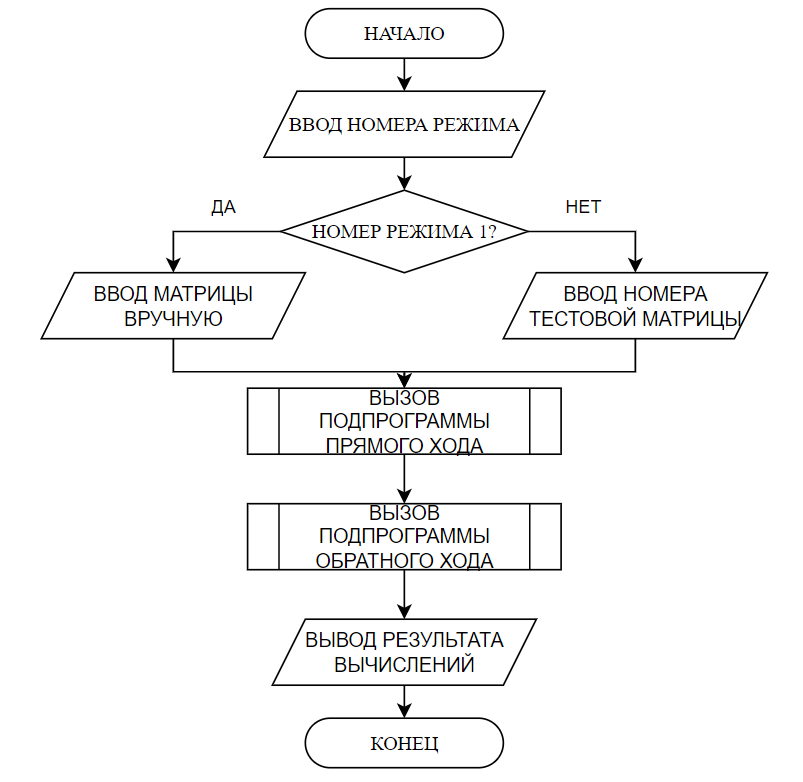
\includegraphics[scale=0.8]{main.png}
    \caption{Выбор режима работы программы.}
    \label{fig:main}
\end{figure}

На блок-схемах на рис.~\ref{fig:straight} и рис.~\ref{fig:ladder} представленных ниже показано все, что касается первого этапа решения уравнения, а именно прямой проход.

\begin{figure}[H]
    \centering
    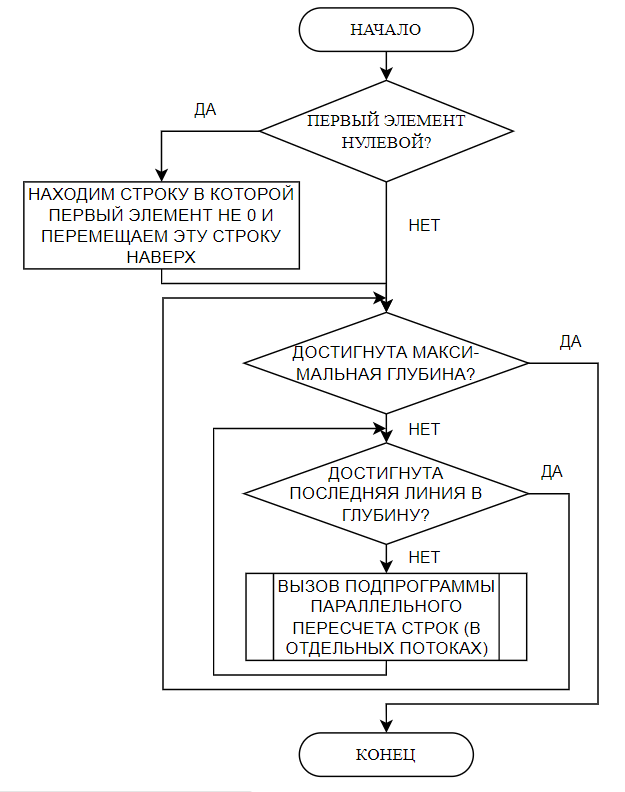
\includegraphics[scale=0.9]{straight.png}
    \caption{Блок-схема для этапа прямого хода решения СЛАУ.}
    \label{fig:straight}
\end{figure}

\begin{figure}[H]
    \centering
    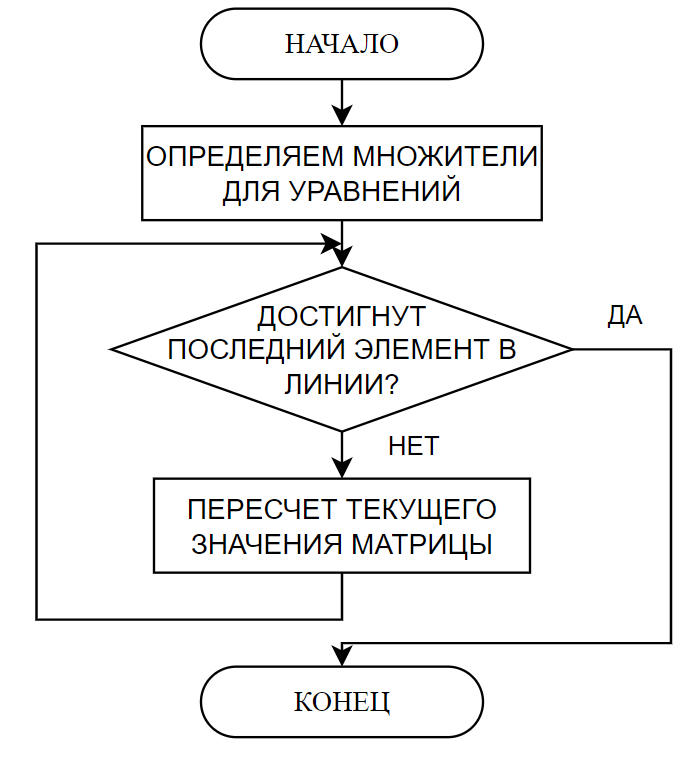
\includegraphics[scale=0.5]{ladder.png}
    \caption{Подпрограмма для параллельного суммирования i-го уравнения с первым уравнением.}
    \label{fig:ladder}
\end{figure}

На рис.~\ref{fig:reverse} и рис.~\ref{fig:rev_ladder} представлены блок-схемы для иллюстрации второго этапа решения СЛАУ, а именно обратного хода решения матрицы.

\begin{figure}[H]
    \centering
    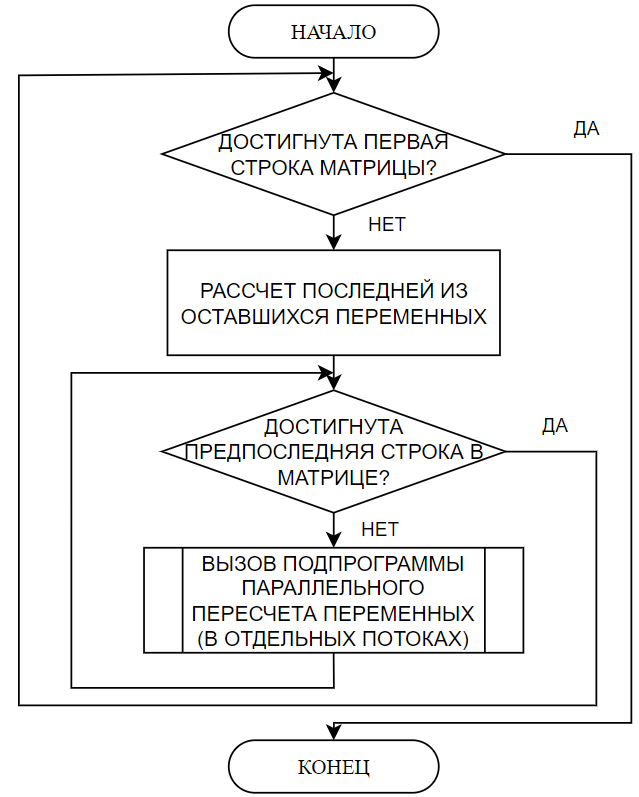
\includegraphics[scale=0.7]{reverse.png}
    \caption{Блок-схема для этапа обратного хода решения СЛАУ.}
    \label{fig:reverse}
\end{figure}

\begin{figure}[H]
    \centering
    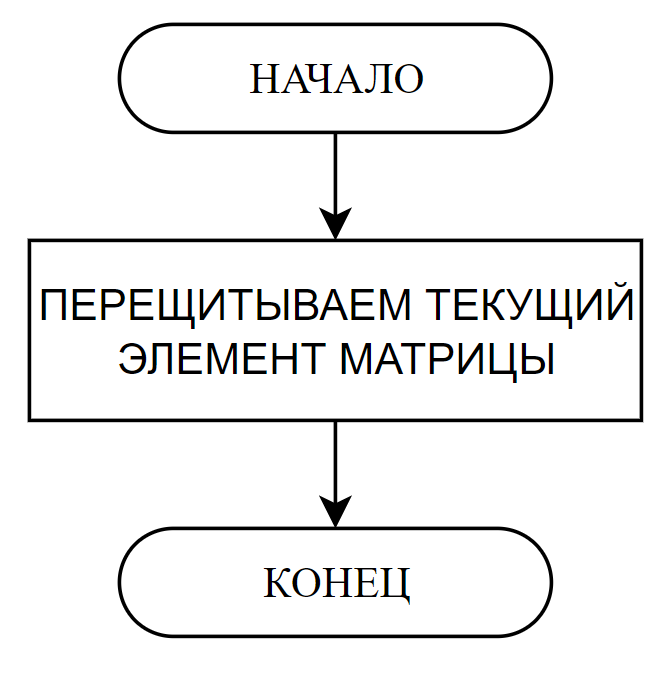
\includegraphics[scale=0.4]{reverse_ladder.png}
    \caption{Подпрограмма для параллельного обновления значений переменных всех столбцов матрицы.}
    \label{fig:rev_ladder}
\end{figure}

\section*{Тестирование работоспособности программы}
\addcontentsline{toc}{section}{Тестирование работоспособности программы}

Для тестирования работоспособности программы предусмотрен отдельный режим, где можно выбрать одну из пяти СЛАУ, для которой можно сравнить результат работы программы с правильным ответом.

В качестве примера для подтверждения работоспособности взята следующая СЛАУ:

\begin{equation*}
    \begin{cases}
        -4x_1 + 6x_2 - 10x_3 - 2x_4 - 2x_5 = -72, 
        \\
        -6x_1 + 4x_2 - 4x_3 - 8x_4 - 9x_5 = -67,
        \\
        7x_1 - 5x_2 - 9x_3 - 7x_4 - 9x_5 = -51,
        \\
        x_1 - 6x_2 + 5x_4 - 2x_5 = -44,
        \\
        8x_1 + 4x_2 + 9x_3 + x_4 - 4x_5 = 22.
    \end{cases}
\end{equation*}

На первом этапе нужно привести матрицу к ступенчатому виду. Поскольку первый элемент первой строки не нулевой, то никаких перестановок не требуется. Поэтому нужно нужно последовательно суммировать все уравнения, начиная со второго, с первым таким образом, чтобы получить все нули в первом столбце (для всех уравнений, кроме первого), затем для полученной системы складывать все уравнения, начиная с третьего, со вторым, чтобы получить нули во всех строках ниже второй и т.д.

Результат, полученный после выполнения первого этапа:

\begin{equation*}
    \begin{cases}
        -2x_1 + 3x_2 - 5x_3 - x_4 - x_5 = -36, 
        \\
                5x_2 - 11x_3 + 5x_4 + 6x_5 = -41,
        \\
                       144x_3 + 160x_4 + 191x_5 = 1319,
        \\
                              1640x_4 - 1393x_5 = -1057,
        \\
                                     x_5 = 9.
    \end{cases}
\end{equation*}

На втором этапе нужно раскрутить полученную систему в обратную сторону. Уже известно значение переменной $x_5$, а значит его можно последовательно подставлять в уравнения выше и находить остальные неизвестные коэффициенты.

Правильным ответом в ходе решения этой СЛАУ являются следующие значения: $x_1 = 3$, $x_2 = -1$, $x_3 = 5$, $x_4 = -7$, $x_5 = 9$.

Ниже представлен скриншот работы программы для данной системы уравнений. На выход программы поступает матрица, которая составлена на основе приведенной СЛАУ; список с полученными значениями переменных; время выполнения скрипта.

\begin{figure}[H]
    \centering
    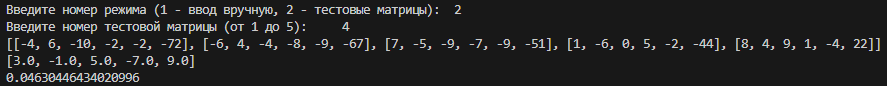
\includegraphics[scale=0.7]{result.png}
    \caption{Результат работы программы для тестовой СЛАУ.}
    \label{fig:result}
\end{figure}

\section*{Вывод}
\addcontentsline{toc}{section}{Вывод}

В ходе выполнения работы было осуществлено знакомство с методом Гаусса для решения СЛАУ и создана и протестирована его программная реализация.

\newpage
\chapter*{\begin{flushright}Приложение\end{flushright}}
\addcontentsline{toc}{chapter}{Приложение}

\begin{code}
\captionof{listing}{\label{code:gauss}Исходный код для решения СЛАУ методом Гаусса.}
\vspace{0.5cm}
{\small
\inputminted[mathescape,linenos,frame=lines,breaklines]{Python}{gauss.py}
}
\end{code}

\end{document}
